As we have observed in the earlier chapters, an efficient program is one that makes full use of the available hardware resources and does not waste them for tasks that are not needed. A high-performing program cannot be described so simply because performance can be defined only with respect to specific targets. Nonetheless, in this book, and in particular, in this chapter, we are largely concerned with the computational performance or throughput: how fast can we solve a given problem with the hardware resources we have? This type of performance is closely related to efficiency: our program will deliver the result faster if every computation it executes brings us closer to the result, and, at every moment, we do as much computing as possible.

This brings us to the next question: just how much computing can be done, say, in one second? The answer, of course, will depend on what hardware you have, how much of it, and how efficiently your program can use it. Any program needs multiple hardware components: processors and memory, obviously, but also networking for any distributed program, storage, and other I/O channels for any program that manipulates large amounts of external data, possibly other hardware, depending on what the program does. But everything starts with the processor, and so, perforce, does our exploration of high-performance programming. Furthermore, in this chapter, we will limit ourselves to a single thread of execution; concurrency will come later.

With this narrower focus, we can define what this chapter is about: how to make the best use of the CPU resources using a single thread. To understand this, we first need to explore what are the resources that a CPU has. Of course, different generations and different models of processors will have a different assortment of hardware capabilities, but the goal of this book is two-fold: first, to give you a general understanding of the subject, and second, to equip you with the tools necessary to acquire more detailed and specific knowledge. The general overview of the computational resources available on any modern CPU can be summarized, unfortunately, as it's complicated. To illustrate, consider this die image of an Intel CPU:

\hspace*{\fill} \\ %插入空行
\begin{center}
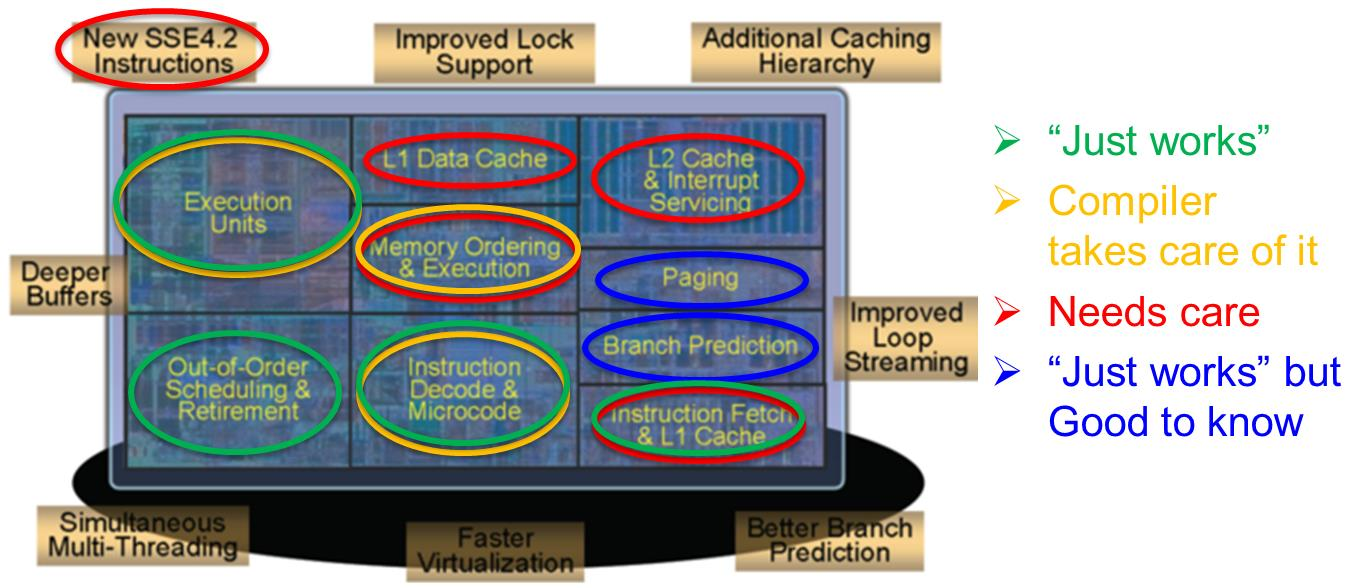
\includegraphics[width=0.9\textwidth]{content/1/chapter3/images/1.jpg}\\
Figure 3.1 – Die image of a Pentium CPU, with the markup of functional areas (source: Intel)
\end{center}

Overlaid on top of the image are the descriptions of the major functional areas. If this is the first time you have seen such an image, the most startling detail may be that the execution unit, that is, the part that does actual additions, multiplications, and other operations that we think of as the main function of the CPU, actually doesn't take up even a quarter of all the silicon. The rest is other stuff whose purpose is, fundamentally, to enable the additions and multiplications to work and work efficiently. The second and more practically relevant observation is this: the processor has many components with different functions. Some of these components largely work by themselves, and there is little the programmer needs to do to make the best use of them. Some need a careful arrangement of the machine code that, thankfully, is mostly done by the compilers. But more than half of the silicon area is dedicated to the components that don't just optimize themselves: to get the maximum performance out of this processor, the programmer needs to understand how they work, what they can and cannot do, and what affects the efficiency of their operations (both positively and negatively). Often even the parts that work OK by themselves can benefit from the programmer's attention if truly exceptional performance is desired.

There are many books written on processor architecture, including all the hardware techniques the designers use to improve the performance of their creations. These books can be a source of valuable knowledge and understanding. This is not going to be yet another one of those books. What descriptions and explanations of the hardware it does have, serve a different goal: here, we will focus on the practical ways in which you can explore the performance of your hardware, starting with the CPUs. We start this exploration without delay in the next section.













































